	A Figura \ref{fig:questao5_LGR&Ganho_sistema_nao_compensado}  mostra o LGR e o ganho para o sistema n�o compensado. A partir do Gr�fico, foi obtido os valores que seguem na tabela \ref{tab:valoresq4}. O sistema n�o compensado est� na Figura \ref{fig:funcaotransferencianaocompensado}.
	
	\begin{figure}[h!]
		\centering
		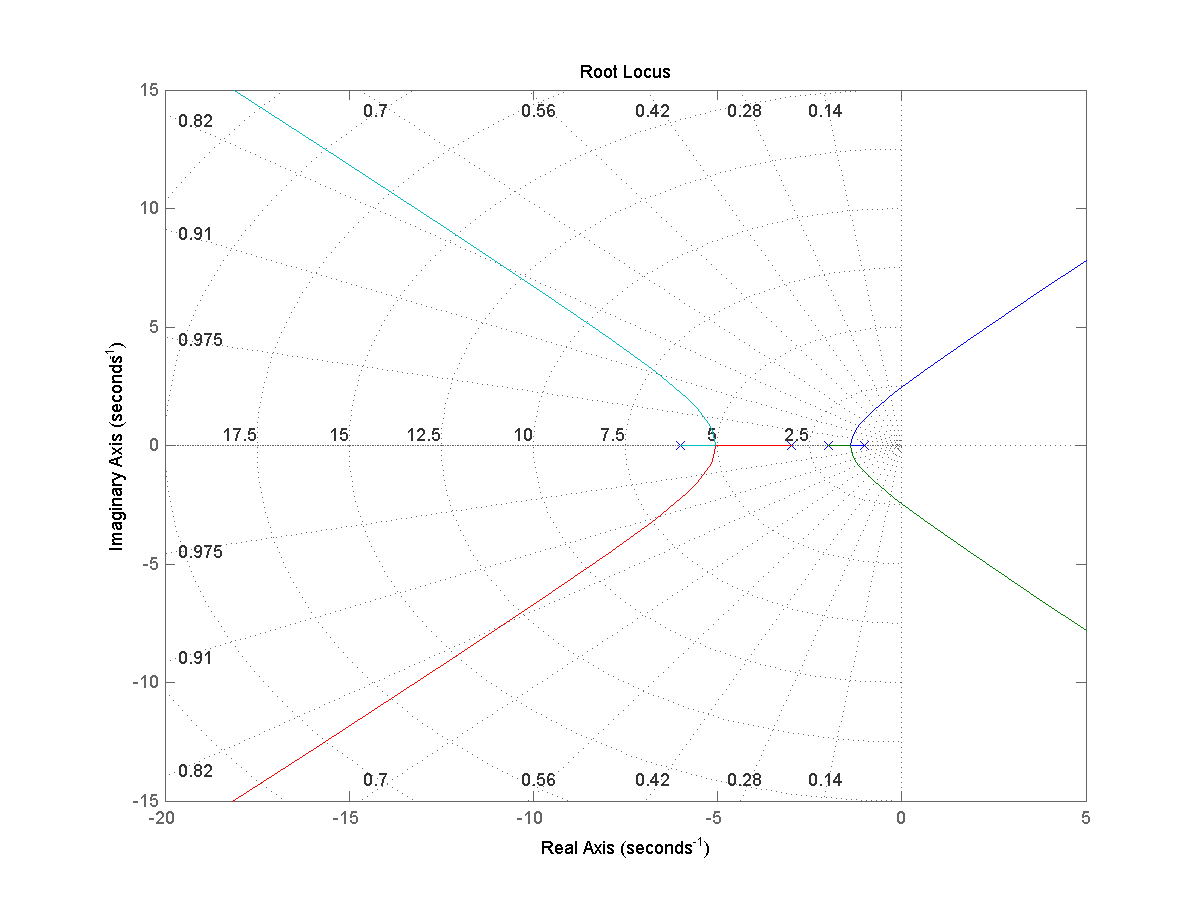
\includegraphics[scale=0.6]{./questao4/lgrq4naocompensado.png}
		\caption{LGR do sistema n�o compensado}		
		\label{fig:lgrq4naocompensado}
	\end{figure}

	\begin{figure}[h!]
		\centering
		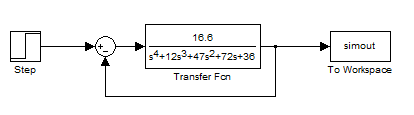
\includegraphics[scale=0.6]{./questao4/funcaotransferencianaocompensado.png}
		\caption{Sistema n�o compensado}		
		\label{fig:funcaotransferencianaocompensado}
	\end{figure}
	
	Usando o valor original do $T_{s}$ encontrado na simula��o, encontra-se um novo $T_{s_{2\%}}$ por:
	
	\[ T_{s} = \frac{4,454}{2} = 2,227 \rightarrow T_{s} = \frac{4}{\sigma} \rightarrow \sigma = \frac{4}{2,227} = 1,7961 \]
	
	A partir do $\sigma$, tem-se a parte real do novo polo dominante e deve-se calcular a parte imagin�ria por:
	
	\[ \sigma = \xi W_{n} \rightarrow W_{n} = \frac{\sigma}{\xi} = \frac{1,7961}{0,707} = 2,5404 \]
	
	Obtido o valor de $W_{n}$, a parte imagin�ria � calculada por:
	
	\[ W_{d} = W_{n} \sqrt{1 - \xi} = 2,5404 \sqrt{1 -0,707} = 1,7961  \] 
	
	Dado o novo polo dominante em $-1,7961 + 1,7961i$, deve ser achar o �ngulo que o novo zero a ser inserido far� com o eixo real. Para isto, o c�lculo deste �ngulo � feito por:
	
	\[ \theta_{1} - \theta_{2} - \theta_{3} - \theta_{4} - \theta_{5} = (2k+1)180 \]
	
	Onde: 
	
	\[ \theta_{2} = tg^{-1} \frac{1,7961}{-1,7961 + 1} = 113,9 \]
	
	\[ \theta_{3} = tg^{-1} \frac{1,7961}{-1,7961 + 2} = 83,52 \]
	
	\[ \theta_{4} = tg^{-1} \frac{1,7961}{-1,7961 + 3} = 56,16 \]
	
	\[ \theta_{5} = tg^{-1} \frac{1,7961}{-1,7961 + 6} = 23,13 \]
	
	\[ \theta_{1} = 96,71 \]
	
	Para achar o ponto onde o zero deve ser inserido, deve-se achar a sua dist�ncia em rela��o ao eixo imagin�rio com a equa��o:
	
	\[ \frac{1,7961}{1,7961 - \sigma_{c}} = tg(180 - 96,71) \rightarrow 8,4997\sigma_{c} - 15,2663 = 1,7961 \rightarrow \sigma_{c} = 2,007 \]
	
	O zero deve ser colocado no ponto 2,007. O novo LGR formado se encontra na \ref{fig:lgrq4compensado}. Mantendo-se o mesmo $\xi$, os valores da vari�veis encontradas no LGR est�o na tabela \ref{tab:valoresq4}. O sistema compensado ficou como na Figura \ref{fig:funcaotransferencianaocompensado}. A resposta do sistema est� na Figura \ref{fig:comparacaocompensadoenaocompensado} com o sistema n�o compensado em azul e o compensado em verde.
	
	\begin{figure}[h!]
		\centering
		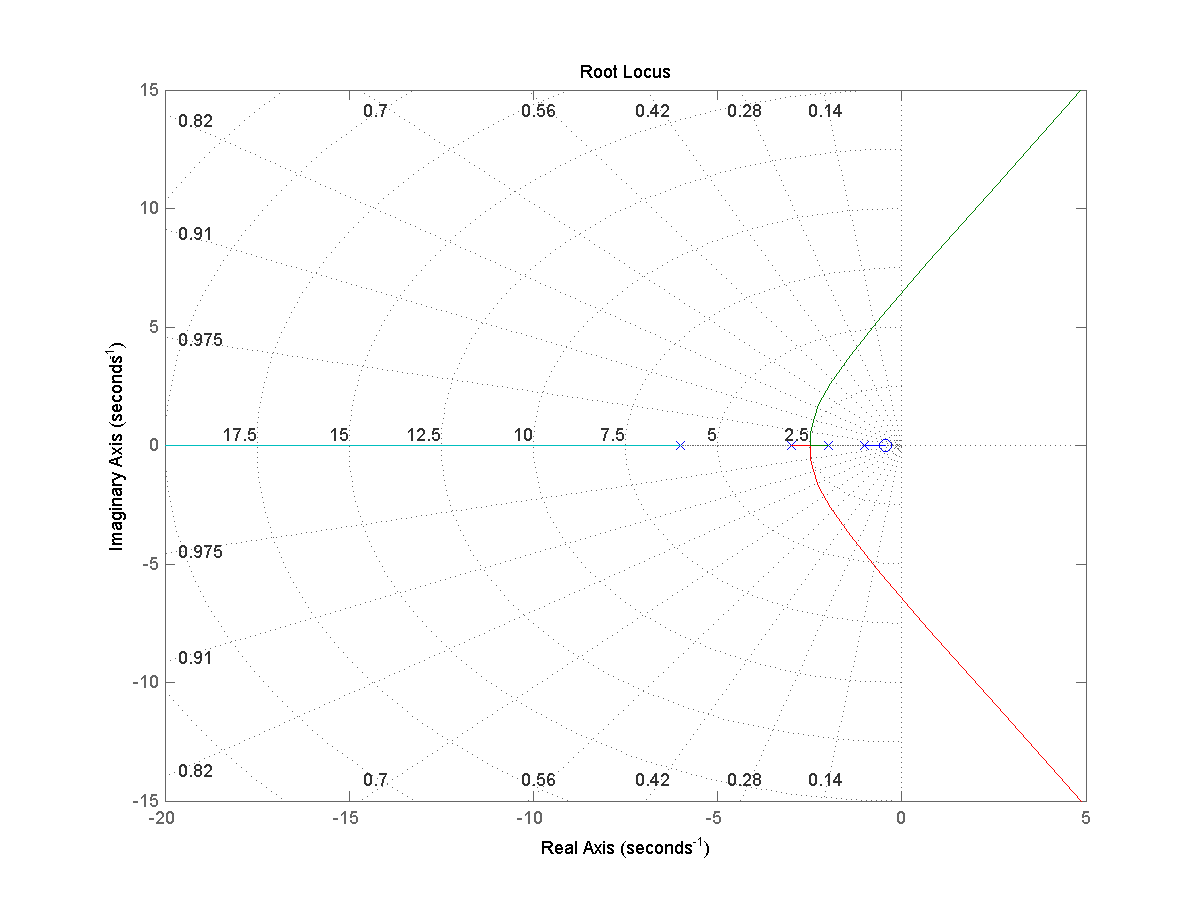
\includegraphics[scale=0.6]{./questao4/lgrq4compensado.png}
		\caption{LGR do sistema compensado}		
		\label{fig:lgrq4compensado}
	\end{figure}

	\begin{table}
		\centering
		\begin{tabular}{|c|c|c|}
		\hline
		Vari�vel & N�o compensado & Compensado \\
		\hline
		$\xi$ & 0,707 & 0,707 \\
		\hline
		Ganho & 16,6 & 19,2 \\
		\hline
		Polo Dominante & -1,04 + 1,04i & -2,12 + 2,12i \\
		\hline
		$W_{n}$ & 1,47 & 3 \\
		\hline
		$V_{r}$ & 0,3156 & 0,517 \\
		\hline
		$T_{p}$ & 0,3531 & 0,5437 \\
		\hline
		$T_{s}$ & 2,737 & 4,454 \\
		\hline
		\end{tabular}
		\caption{Valores extra�dos dos LGRs e das respostas do sistemas compensados e n�o compensados na simula��o}
		\label{tab:valoresq4}
	\end{table}
	
	\begin{figure}[h!]
		\centering
		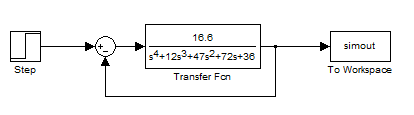
\includegraphics[scale=0.6]{./questao4/funcaotransferencianaocompensado.png}
		\caption{Sistema n�o compensado}		
		\label{fig:funcaotransferencianaocompensado}
	\end{figure}
	
	\begin{figure}[h!]
		\centering
		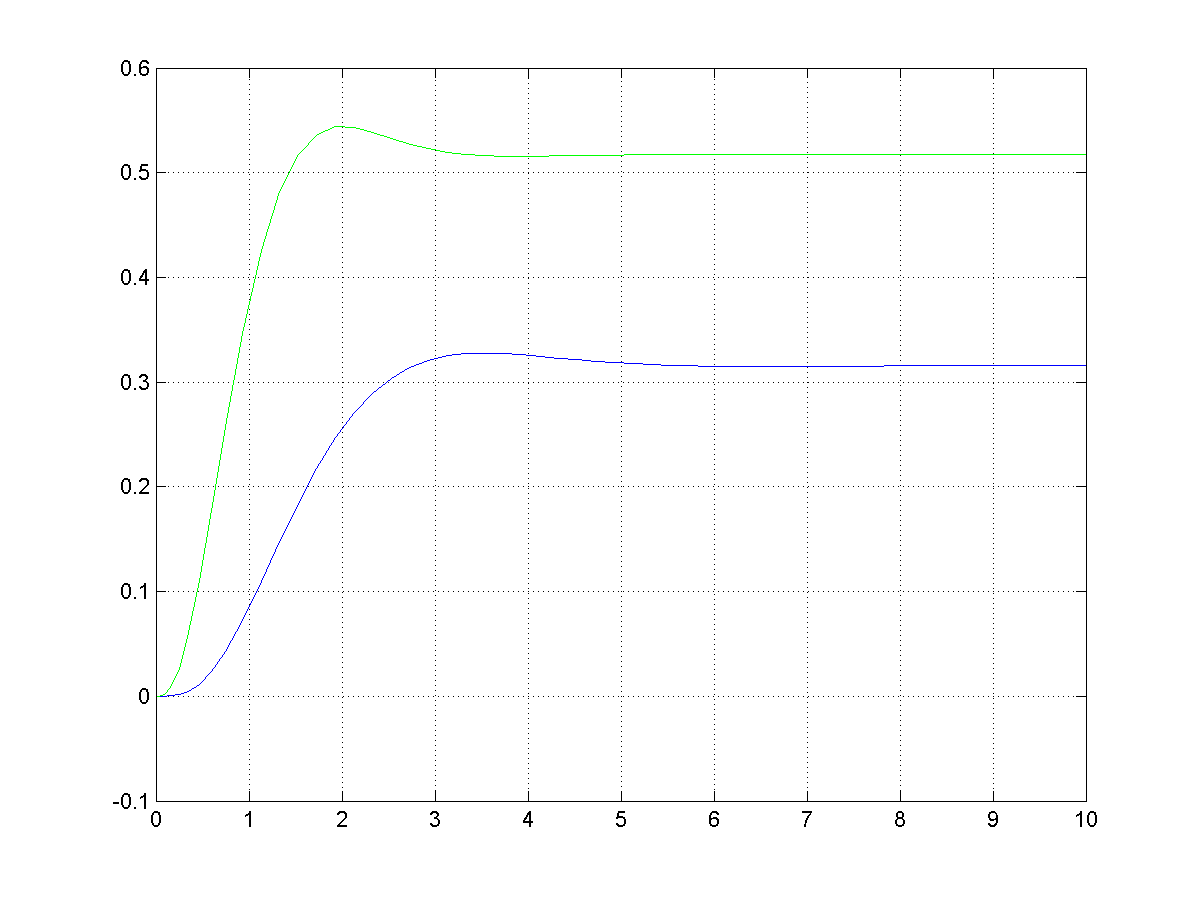
\includegraphics[scale=0.6]{./questao4/comparacaocompensadoenaocompensado.png}
		\caption{Compara��o da resposta do sistema n�o compensado em azul e do sistema compensado em verde}		
		\label{fig:comparacaocompensadoenaocompensado}
	\end{figure}